\documentclass[12pt,letterpaper, onecolumn]{exam}
\usepackage{graphicx}
\usepackage{caption}
\usepackage{color}
\usepackage{caption}
\usepackage{listings}
\usepackage[dvipsnames]{xcolor}
\graphicspath{ {./images/} }
\lhead{Mustafa Rashid\\}
\rhead{Homework 4a: Extra Credit Assignment\\}
\chead{\hline} 
\thispagestyle{empty} 
\newcommand*{\setdef}[1]{\left\{#1 \right\}} 
\renewcommand{\thepartno}{\Alph{partno}} % Force uppercase letters
\renewcommand{\partlabel}{\thepartno.}    % Format as A. B. C.

\begin{document}
\begingroup  
\noindent\LARGE CIS 5500: Database and Information Systems\\
\noindent\LARGE Homework 4a: Extra Credit Assignment\\
\noindent\large \today\\
\noindent\large Mustafa Rashid\par
\noindent\large Spring 2026\par
\endgroup
\rule{\textwidth}{0.4pt}
\pointsdroppedatright
\printanswers
\renewcommand{\solutiontitle}{\noindent\textbf{Ans:}\enspace}

% SQL listing from https://gist.githubusercontent.com/vivngo/e37e1c7b79bf7e8b910c6566c59c46be/raw/db8723fc80c8b1b01665851106dba2f370b5d865/code.tex
\definecolor{dkgreen}{rgb}{0,0.6,0}
\definecolor{gray}{rgb}{0.5,0.5,0.5}
\definecolor{mauve}{rgb}{0.58,0,0.82}
\lstset{language=SQL,
  basicstyle={\small\ttfamily},
  belowskip=3mm,
  breakatwhitespace=true,
  breaklines=true,
  classoffset=0,
  columns=flexible,
  commentstyle=\color{dkgreen},
  framexleftmargin=0.25em,
  frameshape={}{}{}{}, %To remove to vertical lines on left, set `frameshape={}{}{}{}`
  keywordstyle=\color{blue},
  numbers=none, %If you want line numbers, set `numbers=left`
  numberstyle=\tiny\color{gray},
  showstringspaces=false,
  stringstyle=\color{mauve},
  tabsize=3,
  xleftmargin =1em
}

%Javascript listing from https://mysnippets443.wordpress.com/2015/11/28/latex-insert-javascript-code-with-lstlisting-package/

\definecolor{mygreen}{rgb}{0,0.6,0}
\definecolor{mygray}{rgb}{0.5,0.5,0.5}
\definecolor{mymauve}{rgb}{0.58,0,0.82}
 
%Customize a bit the look
\lstset{ %
backgroundcolor=\color{white}, % choose the background color; you must add \usepackage{color} or \usepackage{xcolor}
basicstyle=\footnotesize, % the size of the fonts that are used for the code
breakatwhitespace=false, % sets if automatic breaks should only happen at whitespace
breaklines=true, % sets automatic line breaking
captionpos=b, % sets the caption-position to bottom
commentstyle=\color{mygreen}, % comment style
deletekeywords={...}, % if you want to delete keywords from the given language
escapeinside={\%*}{*)}, % if you want to add LaTeX within your code
extendedchars=true, % lets you use non-ASCII characters; for 8-bits encodings only, does not work with UTF-8
frame=single, % adds a frame around the code
keepspaces=true, % keeps spaces in text, useful for keeping indentation of code (possibly needs columns=flexible)
keywordstyle=\color{blue}, % keyword style
% language=Octave, % the language of the code
morekeywords={*,...}, % if you want to add more keywords to the set
numbers=none, % where to put the line-numbers; possible values are (none, left, right)
numbersep=5pt, % how far the line-numbers are from the code
numberstyle=\tiny\color{mygray}, % the style that is used for the line-numbers
rulecolor=\color{black}, % if not set, the frame-color may be changed on line-breaks within not-black text (e.g. comments (green here))
showspaces=false, % show spaces everywhere adding particular underscores; it overrides 'showstringspaces'
showstringspaces=false, % underline spaces within strings only
showtabs=false, % show tabs within strings adding particular underscores
stepnumber=1, % the step between two line-numbers. If it's 1, each line will be numbered
stringstyle=\color{mymauve}, % string literal style
tabsize=2, % sets default tabsize to 2 spaces
title=\lstname % show the filename of files included with \lstinputlisting; also try caption instead of title
}
%END of listing package%
 
\definecolor{darkgray}{rgb}{.4,.4,.4}
\definecolor{purple}{rgb}{0.65, 0.12, 0.82}
 
%define Javascript language
\lstdefinelanguage{JavaScript}{
keywords={typeof, new, true, false, catch, function, return, null, catch, switch, var, if, in, while, do, else, case, break},
keywordstyle=\color{blue}\bfseries,
ndkeywords={class, export, boolean, throw, implements, import, this},
ndkeywordstyle=\color{darkgray}\bfseries,
identifierstyle=\color{black},
sensitive=false,
comment=[l]{//},
morecomment=[s]{/*}{*/},
commentstyle=\color{purple}\ttfamily,
stringstyle=\color{red}\ttfamily,
morestring=[b]',
morestring=[b]"
}
 
\lstset{
language=JavaScript,
extendedchars=true,
basicstyle=\scriptsize\ttfamily,
showstringspaces=false,
showspaces=false,
numbers=none,
numberstyle=\footnotesize,
numbersep=9pt,
tabsize=2,
breaklines=true,
showtabs=false,
captionpos=b,
xleftmargin=0pt,
xrightmargin=0pt
}
\begin{questions}
  \question \textbf{Question 1 (1 point)}
  \begin{parts}
    \part The two points that are vulnerable are 1) lines 127--130 (\texttt{GET /api/lookup}) and 2) lines 100--108 (\texttt{GET /api/transactions}).

    \textbf{Vulnerable line in \texttt{/api/lookup} (line 130):}
    \begin{lstlisting}[language=JavaScript]
const query = `SELECT full_name, username FROM users WHERE full_name LIKE '%${q}%'`;
    \end{lstlisting}

    \textbf{Vulnerable lines in \texttt{/api/transactions} (lines 100--101, 103--108):}
    \begin{lstlisting}[language=JavaScript]
const order = String(req.query.order || "DESC");
const cols  = String(req.query.cols  || "id, amount, description, created_at");

const query = `
  SELECT ${cols}
  FROM   transactions
  WHERE  from_account = ${acc.id} OR to_account = ${acc.id}
  ORDER  BY ${sort} ${order}
  LIMIT  50
`;
    \end{lstlisting}

    In both cases, user-supplied input is concatenated directly into the SQL string without sanitization or parameterization.

    \part
    \textbf{Endpoint 1: \texttt{GET /api/lookup}}
    \begin{enumerate}
      \item Typed in the Account Lookup search box.
      \item Input: \texttt{'}
      \item Error: \texttt{\{"error":"unrecognized token: \textbackslash"'\textbackslash""\}}
    \end{enumerate}

    \textbf{Endpoint 2: \texttt{GET /api/transactions}}
    \begin{enumerate}
      \item Typed in the Display Fields (Custom Columns) input on the Transactions page.
      \item Input: \texttt{id,}
      \item Error: \texttt{\{"error":"near \textbackslash"FROM\textbackslash": syntax error"\}}
    \end{enumerate}
  \end{parts}
  \pagebreak
  \question \textbf{Question 2 (1 point)}
  \begin{parts}
    \part The following payload was entered in the Custom Columns (Display fields) input on the Transactions page:
    \begin{lstlisting}[language=SQL]
(SELECT group_concat(name || ': ' || sql, ' | ') FROM sqlite_master) as id, amount, description, created_at
    \end{lstlisting}
    This injects a scalar subquery into the \texttt{SELECT} clause that reads from \texttt{sqlite\_master} and concatenates each table's name with its \texttt{CREATE TABLE} statement. The full schema was returned in the \texttt{id} field of each row in the raw API response.

    \part Based on the recovered DDL, the columns of each table are:

    \textbf{\texttt{users}:} \texttt{id}, \texttt{username}, \texttt{password\_hash}, \texttt{full\_name}, \texttt{is\_admin}, \texttt{account\_number}

    \textbf{\texttt{accounts}:} \texttt{id}, \texttt{user\_id}, \texttt{balance}, \texttt{account\_type}

    \textbf{\texttt{transactions}:} \texttt{id}, \texttt{from\_account}, \texttt{to\_account}, \texttt{amount}, \texttt{description}, \texttt{created\_at}
  \end{parts}
  \question \textbf{Question 3 (2 points)}
  \begin{parts}
    \part The three inputs were tested one at a time in the Account Lookup search box:
    \begin{itemize}
      \item \texttt{' UNION SELECT 1 --} --- failed with a syntax error (column count mismatch)
      \item \texttt{' UNION SELECT 1,2 --} --- succeeded, returning \texttt{\{"full\_name":1,"username":2\}} as an extra row
      \item \texttt{' UNION SELECT 1,2,3 --} --- failed with a syntax error (column count mismatch)
    \end{itemize}
    \texttt{' UNION SELECT 1,2 --} succeeded because the original query returns exactly 2 columns (\texttt{full\_name}, \texttt{username}), and a UNION requires both SELECT statements to have the same number of columns.

    \part The following payload was entered in the Account Lookup search box:
    \begin{lstlisting}[language=SQL]
' UNION SELECT full_name, account_number FROM users--
    \end{lstlisting}
    Raw API response:
    \begin{lstlisting}[language=SQL]
[{"full_name":"Daniel Zhao","username":"ACC-1002"},
 {"full_name":"Mayur Naik","username":"ACC-2001"},
 {"full_name":"Robert'); DROP TABLE Students;--","username":"ACC-1001"},
 ...]
    \end{lstlisting}
    Mayur Naik's account number is \textbf{ACC-2001}.

    A UNION injection cannot be performed through the \texttt{cols=} parameter on the Transactions page because \texttt{cols} is injected into the middle of the SELECT clause. The FROM, WHERE, ORDER BY, and LIMIT clauses follow immediately after, making it impossible to terminate the first SELECT statement and append a UNION SELECT.
  \end{parts}

  \question \textbf{Question 4 (2 points)}
  \begin{parts}
    \part The following payload was injected by crafting a URL request directly to \texttt{/api/transactions} with the \texttt{order=} parameter URL-encoded:
    \begin{lstlisting}[language=SQL]
DESC; UPDATE accounts SET balance=1000000 WHERE user_id=1--
    \end{lstlisting}
    This terminates the original SELECT with a semicolon and appends an UPDATE statement. Because \texttt{db.prepare().all()} rejects multiple statements, the server falls back to \texttt{db.exec()}, which executes both statements. Bobby's balance was confirmed as \$1,000,000.00 on the Dashboard.
  \end{parts}

  \question \textbf{Question 5 (1 point)}

  \$1,000,000 was transferred to Mayur Naik's account (ACC-2001) using the Wire Transfer panel.

  \begin{center}
    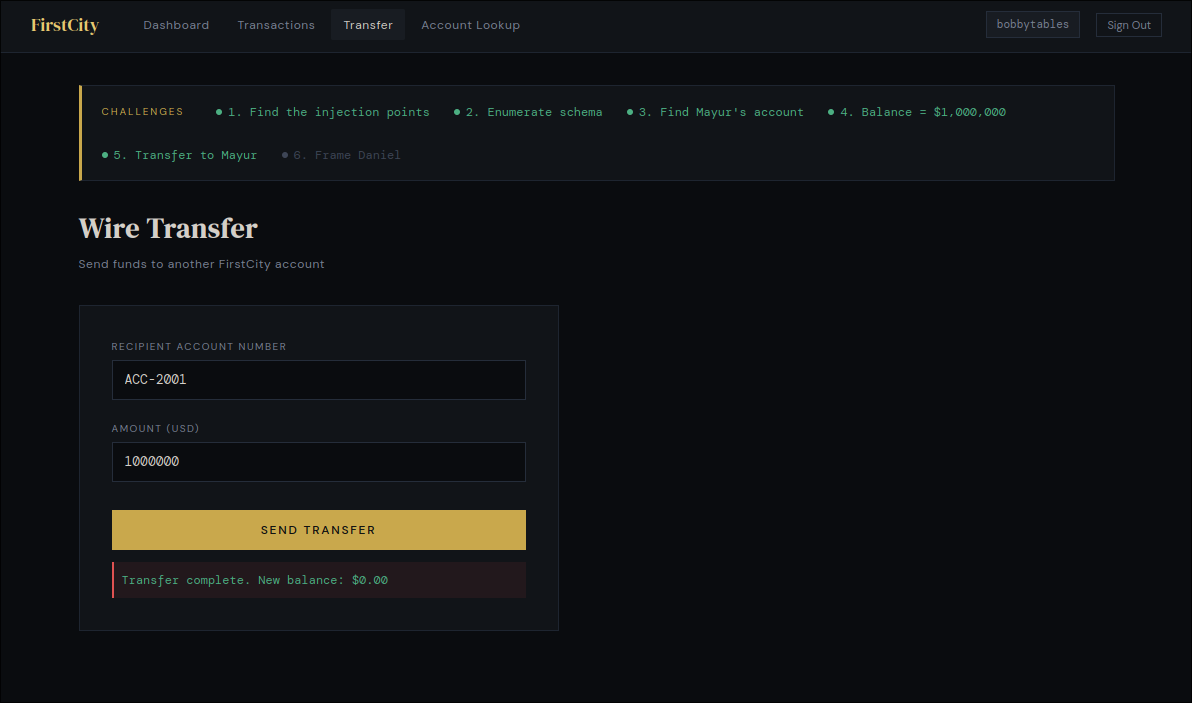
\includegraphics[width=\textwidth]{q5_screenshot}
  \end{center}

  \pagebreak
  \question \textbf{Question 6 (2 points)}
  
  \question \textbf{Question 7 (2 points)}
  \begin{parts}
    \part The corrected JavaScript for both vulnerable endpoints:

    \textbf{Corrected \texttt{GET /api/lookup}:}
    \begin{lstlisting}[language=JavaScript]
app.get("/api/lookup", (req, res) => {
  const q = String(req.query.q || "");
  if (!q) return res.json([]);
  const rows = db.prepare(
    "SELECT full_name, username FROM users WHERE full_name LIKE ?"
  ).all(`%${q}%`);
  return res.json(rows);
});
    \end{lstlisting}

    \textbf{Corrected \texttt{GET /api/transactions}:}
    \begin{lstlisting}[language=JavaScript]
app.get("/api/transactions", requireAuth, (req, res) => {
  const acc = db.prepare(
    "SELECT id FROM accounts WHERE user_id=?"
  ).get(req.session.user_id);

  const allowedSort  = new Set(["amount", "description", "created_at", "id"]);
  const allowedOrder = new Set(["ASC", "DESC"]);
  const sort  = allowedSort.has(String(req.query.sort))
                  ? String(req.query.sort) : "created_at";
  const order = allowedOrder.has(String(req.query.order).toUpperCase())
                  ? String(req.query.order).toUpperCase() : "DESC";

  const query = `
    SELECT id, amount, description, created_at
    FROM   transactions
    WHERE  from_account = ? OR to_account = ?
    ORDER  BY ${sort} ${order}
    LIMIT  50
  `;

  try {
    return res.json(db.prepare(query).all(acc.id, acc.id));
  } catch (e) {
    return res.status(500).json({ error: "An error occurred" });
  }
});
    \end{lstlisting}

    The \texttt{cols} option is removed entirely as it is an inherently unsafe design. \texttt{sort} retains its existing allowlist. \texttt{order} is fixed with an explicit allowlist of \texttt{ASC} and \texttt{DESC}. User input in the \texttt{LIKE} query is passed as a parameterized value, preventing injection.

    \part Leaking raw SQLite error messages is dangerous because they reveal internal database structure to the attacker (table names, column names, and query syntax) which can be used to craft further injections. In Q1B, the error messages directly confirmed both injection points.

    The corrected catch block:
    \begin{lstlisting}[language=JavaScript]
} catch (_) {
  return res.status(500).json({ error: "An error occurred" });
}
    \end{lstlisting}
  \end{parts}
\end{questions}
\end{document}
